\documentclass{article}

\usepackage{graphicx}
\usepackage{tikz}
\usepackage{tikzsymbols}
\usetikzlibrary{calc,patterns,shapes.geometric}
\pagestyle{empty}
\usepackage[margin=0pt]{geometry}
\geometry{papersize={14in,12in}}

\def\centerarc[#1](#2)(#3:#4:#5){\draw[#1] ($(#2)+({#5*cos(#3)},{#5*sin(#3)})$) arc (#3:#4:#5);}

\begin{document}
	\begin{figure}
		\centering
		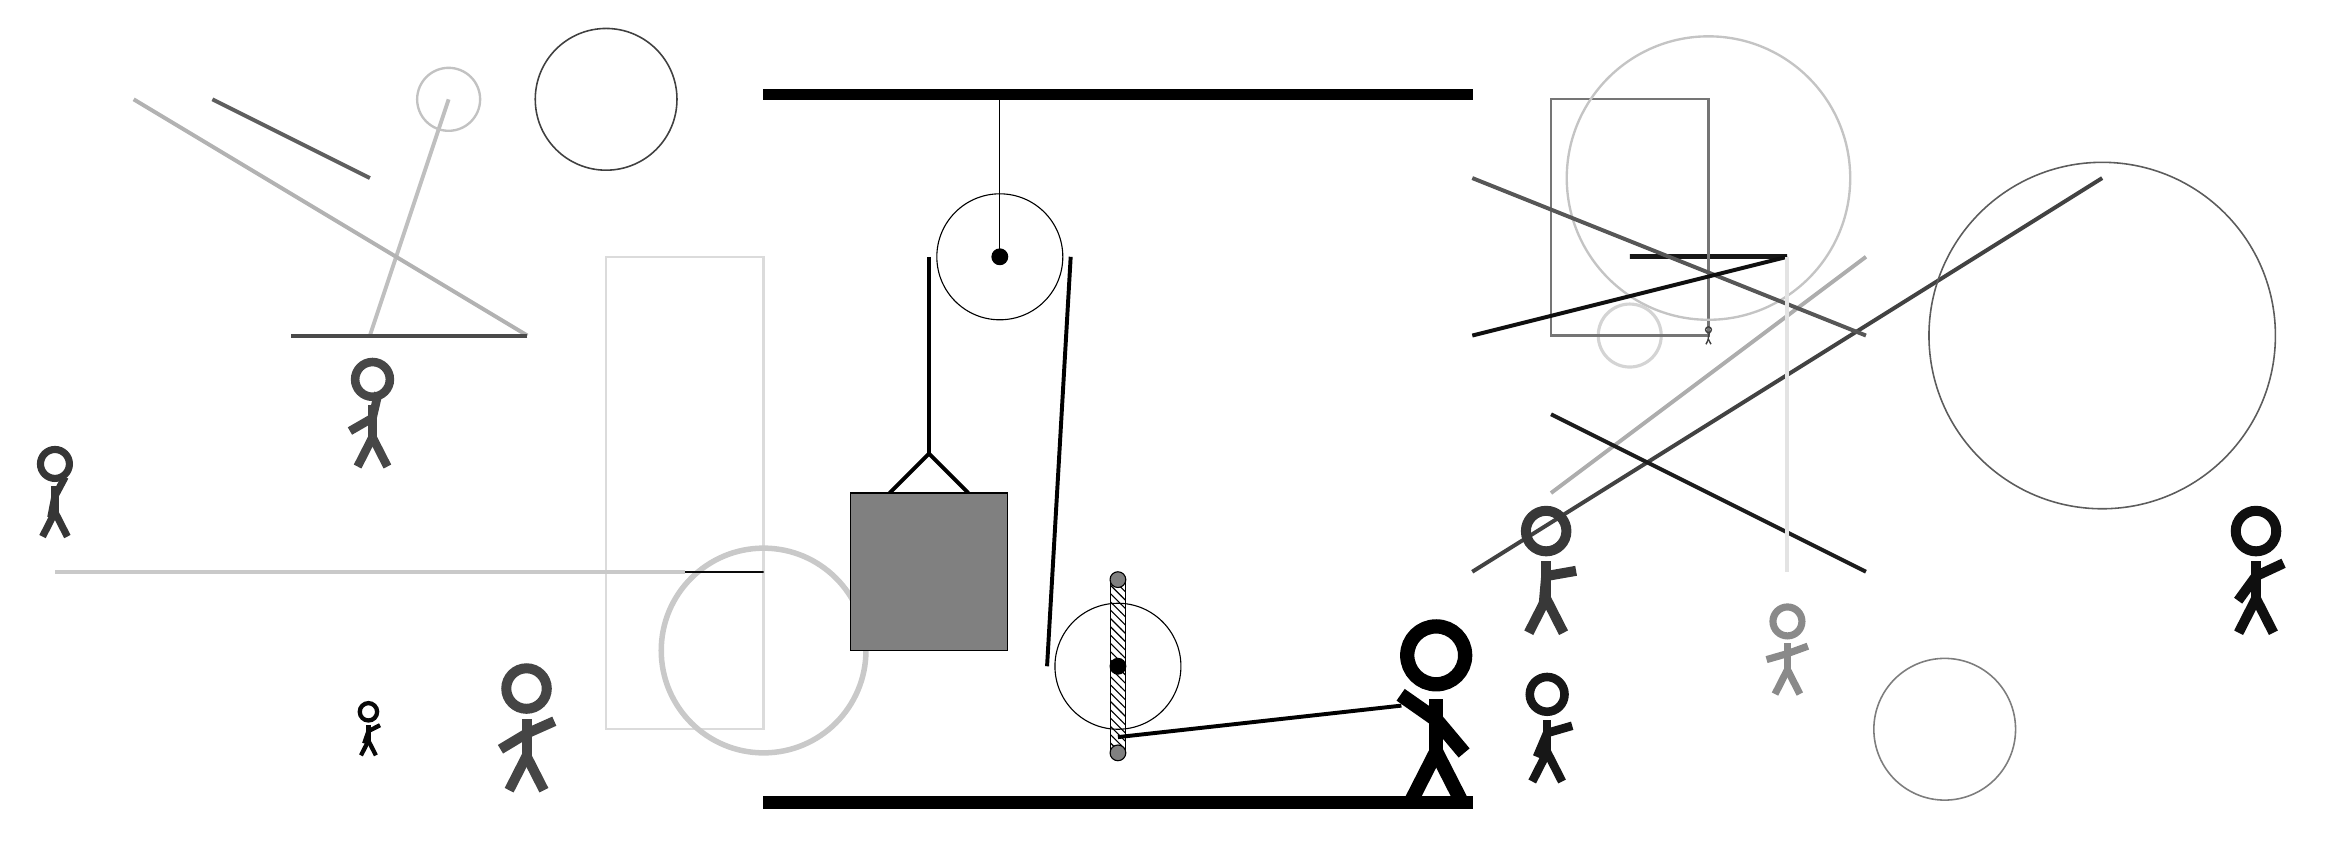
\begin{tikzpicture}
			%%%%% START %%%%%
			
			\draw[fill=black] (-2, 9) rectangle (7, 9.125);
			
			\draw (1, 7) circle (0.8);
			\draw[fill=black] (1, 7) circle (0.1);
			\draw (1, 9) -- (1, 7);
			
			\draw[fill=white](2.5, 1.8) circle (0.8);
			\draw[fill=black] (2.5, 1.8) circle (0.1);
			\draw[pattern=north west lines, pattern color=black] (2.4, 2.9) rectangle (2.6, 0.7);
			\draw[fill=black!50] (2.5, 2.9) circle (0.1);
			\draw[fill=black!50] (2.5, 0.7) circle (0.1);
			
			\draw[line width=0.5mm, color=black!63](-7, 8) -- (-9, 9);
			
			\draw[line width=0.6mm, color=black!91] (9, 7) rectangle (11, 7);
			\draw[line width=0.5mm, color=black!25](-7, 6) -- (-6, 9);
			\node[line width=0.6mm, color=black!91] at (8, 1) {\Strichmaxerl[6][67][16]};
			\draw [line width=0.4mm, color=black!17](9, 6) circle (0.4);
			
			\draw[line width=0.3mm, color=black!54] (8, 6) rectangle (10, 9);
			\draw [line width=0.2mm, color=black!51](13, 1) circle (0.9);
			
			\node[line width=0.2mm, color=black!46] at (11, 2) {\Strichmaxerl[5][16][20]};
			\node[line width=0.4mm, color=black!72] at (-7, 5) {\Strichmaxerl[6][30][77]};
			\draw[line width=0.5mm, color=black!32](12, 7) -- (8, 4);
			
			\draw[line width=0.5mm, color=black!30](-5, 6) -- (-10, 9);
			\draw[line width=0.5mm, color=black!74](7, 3) -- (15, 8);
			\draw [line width=0.3mm, color=black!23](10, 8) circle (1.8);
			\draw [line width=0.2mm, color=black!64](15, 6) circle (2.2);
			\node[line width=0.3mm, color=black!79] at (-11, 4) {\Strichmaxerl[5][79][62]};
			\node[line width=0.2mm, color=black!94] at (17, 3) {\Strichmaxerl[7][54][25]};
			
			\node[line width=0.2mm, color=black!73] at (-5, 1) {\Strichmaxerl[7][31][24]};
			\node[line width=0.4mm, color=black!75] at (10, 6) {\Strichmaxerl[1][84][73]};
			\node[line width=0.5mm, color=black!97] at (-7, 1) {\Strichmaxerl[3][71][27]};
			\draw[line width=0.5mm, color=black!71](-5, 6) -- (-8, 6);
			\draw[line width=0.5mm, color=black!66](12, 6) -- (7, 8);
			
			\draw[line width=0.3mm, color=black!14] (-4, 1) rectangle (-2, 7);
			
			\draw [line width=0.7mm, color=black!21](-2, 2) circle (1.3);
			\draw[line width=0.3mm, color=black!96] (-2, 3) rectangle (-5, 3);
			\node[line width=0.2mm, color=black!78] at (8, 3) {\Strichmaxerl[7][85][10]};
			\draw[line width=0.5mm, color=black!89](8, 5) -- (12, 3);
			
			\draw[line width=0.5mm, color=black!94](11, 7) -- (7, 6);
			\draw[line width=0.5mm, color=black!21](-3, 3) -- (-11, 3);
			\draw [line width=0.2mm, color=black!75](-4, 9) circle (0.9);
			
			\draw[line width=0.5mm, color=black!11](11, 3) -- (11, 7);
			\draw [line width=0.3mm, color=black!24](-6, 9) circle (0.4);
			
			\draw[line width=0.5mm] (-0.4, 4.0) -- (0.1, 4.5) -- (0.6, 4.0);
			\draw[fill=black!50] (-0.9, 4.0) rectangle (1.1, 2.0);
			
			\draw[line width=0.5mm] (0.1, 7) -- (0.1, 4.5);
			\centerarc[line width=0.5mm](1, 7)(0:180:0.9);
			\draw[line width=0.5mm](1.9, 7) -- (1.6, 1.8);
			\centerarc[line width=0.5mm](2.5, 1.8)(180:270:0.9);
			\draw[line width=0.5mm](2.5, 0.9) -- (6.1, 1.3);
			
			\node at (6.5, 1.2) {\Strichmaxerl[10][-35][-50]};
			
			\draw[fill=black] (-2, 0) rectangle (7, 0.15);
			
			%%%%% END %%%%%
		\end{tikzpicture}
	\end{figure}	
\end{document}